\documentclass[10pt,twocolumn]{article}
\usepackage{simpleConference}
\usepackage{times}
\usepackage{float}
\usepackage{graphicx}
\usepackage{hyperref}
\usepackage{mdwlist}
\usepackage{amssymb}
\usepackage{amsmath}
  
\title{Wiisel}
\author{Team: Hala Diab, Sam Friedman, Joe Wright\\
\\
EECS 149 Project Report\\
19 December 2014\\
University of California, Berkeley}
%\date{19 December - EE C149 Fall 2014}

\begin{document}
\maketitle
\thispagestyle{empty}
\begin{abstract}
    A user will be able to use a Nintendo Wiimote to draw on a large screen of
LEDs in a variety of colors. The user will also be able to switch to display mode for a slide show of bitmap images.
\end{abstract}

\section{Model}
We modeled our system as a finite-state machine (in Figure \ref{fsm}). The FSM
models how a user interacting with a Wiimote changes what is on the display.
The model doesn't have a sense of which pixels are set (such an FSM would be
\textit{very} large and complicated, and not terribly useful for the system
design). Each state represents an abstract idea of setting a pixel (whose
position is determined by Wiimote sensor data and is not captured by the
model), setting the entire display to preset pixel data, clearing a pixel,
clearing the entire array, and swapping pointer color.

\section{\textbf{System Structure}}

%\begin{figure}[H]
    %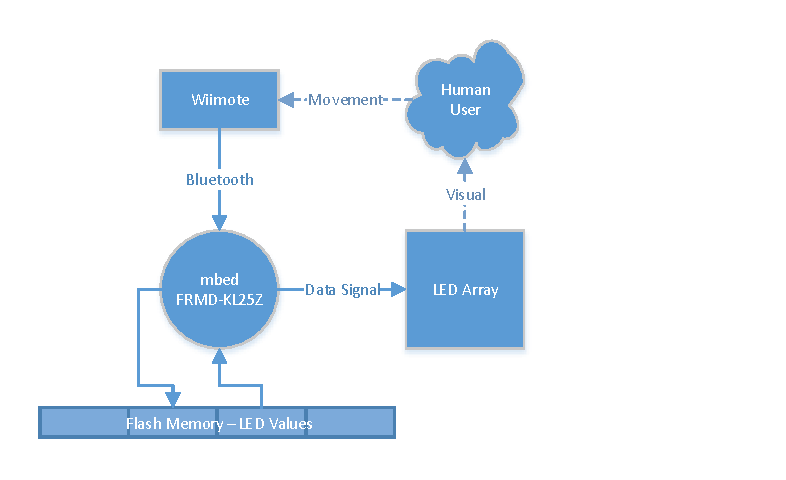
\includegraphics[trim=1cm 0cm 4cm 0cm, width=\linewidth]{dataflow.pdf}
    %\caption{Data Flow and Project Structure}
%\end{figure}
Generally, A user will use a Nintendo Wiimote to communicate sensor data via
Bluetooth to a microprocessor, which in turn controls the array of LEDs. 
Figure \ref{detailed-data-flow} shows more details about the interaction between Wiimote, Screen, and the microprocessor.
\begin{figure}[H]
    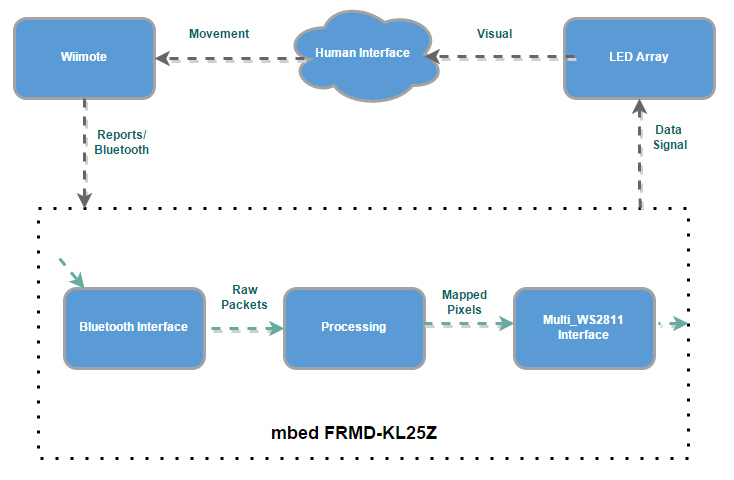
\includegraphics[trim=3cm 0cm 4cm 0cm, width=2.5in]{dataflow1.png}
    \caption{Detailed Data Flow}
    \label{detailed-data-flow}
\end{figure}
\section{\textbf{System Components}}
Components were, in general, selected for their ``embedded'' character, cost, and minimal
feature sets.
\subsection{Screen of WS2812b LEDs}
The screen is 1 meter by 1 meter, with a 30x30 resolution, and
is made of WS2812b individually addressable LEDs. It consists of: 15 strips
with 30 LEDs per strip and 15 strips with 60 LEDs per strip. Two 74HCT245
buffer chips allow the 3.3V logic of the microcontroller to effectively
control the LEDs, which require a minimum data signal voltage of 70\% of the
power supply voltage.
\subsection{Freescale mbed FRDM-KL25Z}
We selected the mbed FRDM-KL25Z; 32-bit ARM Cortex microcontroller that runs
at 48MHz, has 128kB of Flash storage for code, 16kB of RAM for variables. The
FRDM-KL25Z is very low cost, and the low amount of memory required lots of
code optimization and modification to existing libraries to drive all 1,350
LEDs. Another candidate was the Teensy
3.1\footnote{\url{http://www.pjrc.com/teensy/index.html}}, which is very
popular for people building large arrays out of WS2812-based LEDs. We decided
against it for three reasons: it is slightly more expensive, it does not have
USB-host software support (although the hardware can, in theory, support it),
and it was far more powerful than what we needed (and in our view, went
against the spirit of working on an embedded system).
\subsection{Wiimote}
The Nintendo Wiimote is the sensor platform. This includes a 3-axis
accelerometer and several buttons. The Wiimote interfaces with the
microcontroller over bluetooth using a Bluetooth CSR 4.0 USB dongle that is
connected to the microcontroller using USB OTG. The Wiimote make sense as a
sensor platform and user interface, because it is simple, easy to communicate
with, and readily available.
\section{\textbf{Building the System}}
The hardware is designed to be modular so that it can be set up and taken down
in a reasonable amount of time. It also allows damaged or defective strips of
LEDs to be replaced with minimal work. We found that the LEDs had a fairly
high defective rate; our final display ended up with 2-3 dead pixels and we
had to replace a half-row of LEDs that didn't work entirely.
\begin{figure}[H]
    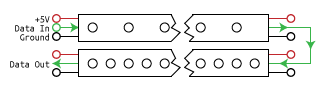
\includegraphics[width=3.5in]{Wiring_Diagram.png}
    \caption{LED Strip Wiring}
    \label{wiring-diagram}
\end{figure}
Figure \ref{wiring-diagram} shows how two LED strips are connected. A single
GPIO pin controls 90 LEDs. In the second strip (with 60 LEDs per meter), every
other LED is set to ``off'' so that the display maintains a constant, uniform
30x30 resolution. This mapping is handled via software, and although currently
hard-coded, could easily be adapted for any arrangement or configuration of
LEDs. Each set of two rows has their power and ground lines connected, so a
single data line addresses two rows, while a single power line powers four.
The data lines are made of CAT-5e networking cables. This allows them to be
easily disconnected from the microcontroller. Additionally, each twisted-pair
has a data line and a ground that terminates at the same end of the same
strip. This helps reduce interference. Between the 74HTC245 buffer chip and
data lines are 100-ohm resistors, which match the impedence of the CAT-5e
cables. This further helps with noise reduction.
\section{\textbf{Software}}
\subsection{Screen Control}
To control the LEDs, we are using the Multi\_WS2811 library\footnote{This
library is by Ned Konz for the FRDM-KL25Z, and is made available to us under
the Apache License.} This library can control up to 16 strips of LEDs in
parallel using 3-phase DMA transfers. The number of parallel LED
strips is limited to at most the number of pins on a single GPIO port for the
microcontroller. 
\subsection{Wiimote}
Data Packets from Wiimote are reported over Bluetooth to the mbed where it
processes the packets using a bluetooth stack built on top of a USB software interface:
\begin{enumerate*}
    \item
        \textbf{KL46Z-USBHost}\footnote{\url{http://developer.mbed.org/users/va009039/code/KL46Z-USBHost/}}:
a simple USBHost library for FRDM-KL46Z(FRDM-KL25Z) by Norimasa Okamoto, under MIT and Apache license.
\item
    \textbf{KL46Z-BTstack}\footnote{\url{http://developer.mbed.org/users/va009039/code/KL46Z-BTstack_example/}}:
a Bluetooth Stack (built on top of KL46Z-USBHost) by Norimasa Okamoto. Supports L2CAP protocol used by the Wiimote.
\end{enumerate*}
We processed packets to extract acceleration and buttons values. To get
accurate acceleration values, we had to calibrate the wiimote we used.
Assuming that bias and sensitivity are roughly equal along all axes, we
modeled wiimote as an affine model: $f(x) = 102x + 486 $. Wiimote calibration
cannot currently be done without recompiling and deploying software, but that
is a possible area for future development.
Roll and pitch were calculated using following equations\footnote{Source:Implementing a Tilt-Compensated eCompass using Accelerometer and Magnetometer Sensors by Talat Ozyagcilar}:
\begin{align*}
    \mathrm{roll} &= \arctan \left ( \frac{x}{z}\right)  \\
    \mathrm{pitch} &= \arctan \left (\frac{y}{x \sin(\mathrm{roll}) + z
    \cos(\mathrm{roll})}\right)
\end{align*}
\section{\textbf{Testing and Verification}} 
We started testing in early phases in the project. We started by testing
screen control software on individual LED strips to confirm that data signals
are sent correctly from microcontroller to strips. This and the difference
between power connection and the daisy chaining of data wires made it easier
to test hardware issues.\\
We encounterd a problem where occasionally a vertical line would appear on the
screen, seemingly randomly. We tested the quality of the signal, used a logic
analyzer to look at the clock timing, and eventually managed to capture a
sequence of 24 bits on an oscillioscope corresponding to an LED affected by
this bug. (Lucky, since there are a lot of bits on any given data line, and
the oscillioscope can either see a large range of data at too-low a resolution
to be useful, or at most two LEDs worth of signal data at a higher
resolution!) We found that a single bit had slightly erratic timing. While the
signal high at the start of a zero-bit should last at most 400 nanoseconds,
with an acceptable error of about 150 nanoseconds, it would
occasionally last over 550 nanoseconds. The offending bit is on the
far right in figure \ref{oscope}.
\begin{figure}[H]
    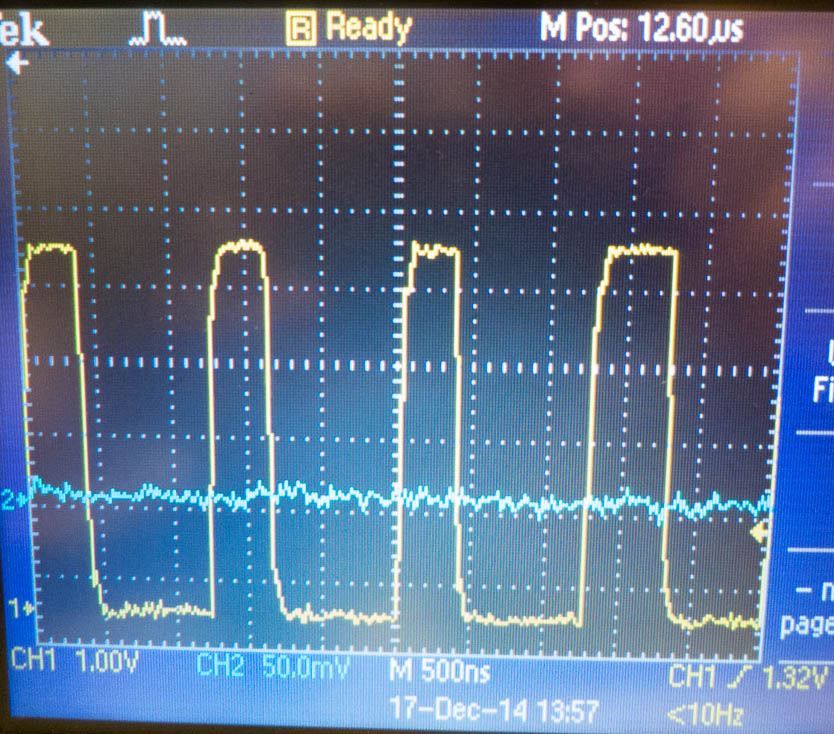
\includegraphics[width=3.5in]{oscope.jpg}
    \caption{Oscillioscope Output}
    \label{oscope}
\end{figure}
The error was entirely eliminated when we reduced the DMA timer to last 300 ns instead
of 400 ns. We suspect that the extra time added to certain bits was a result
of either the USB or Bluetooth library interfering with DMA, or a hardware
problem with the mbed board.
\section{\textbf{Analysis}}
\subsection{Power}
Although datasheets for the specific model of LED strips we have were not
available, a common upper-bound\footnote{This occurs when the LED is set to
full brightness white. Average consumption is much lower} for WS2812b-based 
LEDs is 60 mA per LED\footnote{Burgess, Phillip.``Powering NeoPixels.''
    \textit{Adafruit}. 30 Aug 2013. Web.
    \url{https://learn.adafruit.com/adafruit-
    neopixel-uberguide/power}}. Average-case current draw is typically around
    20 mA. For an array of 900 LEDs, this comes out to a total current draw
    from 18 A to 54 A at 5 volts. \\
    \indent To make the system as safe as possible, we designed the
    LED array hardware to distribute this current evenly and easily
    handle peak usage without catching fire. We also drastically lowered the ``Peak usage'' by limiting the LED brightness in software, and designing the
    system behavior to reduce the frequency of high current draw
    states.\footnote{The default ``blank'' screen is non-white. If the LEDs are off
        instead of white, then initially the array will use very little power,
    instead of the maximum possible.}
    We measured power values and found that we consume 93 W when screen is Red
    with full brightness. Changing mode to 15\% brightness, power consumption
    is decreased to 37 W. The highest power we were able to get the screen to
    consume under normal usage was 42 watts. This
    corresponds to (not including power losses from the 120V AC to 5V DC
    supply) a maximum of 8.4 amps of current, which is less than one-sixth of
    the recommended limit for the wire gauges used in the power distribution
    system.

\subsection{Memory Usage}
As initially written, Multi\_WS2811 library cannot support the number of LEDs
per strip that we need it to in the available amount of RAM on the device. At
80 LEDs per strip, the library takes approximately 98\% of the RAM on the
microcontroller. To remedy this, we moved a large run-time constant array from
RAM to Flash\footnote{The downside to this approach is that we must now
    hardcode all values of the array instead of using \texttt{memset}, which
requires more work on the part of the programmer, but does not affect
functionality of the library.}, which reduced RAM usage to 57\% at 90 LEDs per
strip. We also compressed the color representation from 24 bits per pixel to 
12 bits per pixel.

\section{Future Work}
Adding additional sensors to improve the drawing experience and accuracy is a
possible area of expansion. The Wiimote includes an infrared camera, so
strategically placing IR LEDs on the display can make it possible to compute
the Wiimote's yaw, allowing a user to directly point the Wiimote at the
desired cursor location. There is also a lot more features that can be added
to the Wiisel. Things like changing brush size,
displaying text, saving drawn pictures to an SD card, and displaying arbitary
bitmap images are all features that would make for a better user experience.
However, significant feature expansions would likely require a microcontroller
with a larger amount of memory; the FRDM-KL25Z's memory is almost entirely
used up in the current implementation, with only around 800 bytes free at
peak-usage.

\section{Fun Stats}
\begin{enumerate}
    \item 134 connections crimped
    \item 350 solder joints
\end{enumerate}

\appendix

\begin{figure*}
    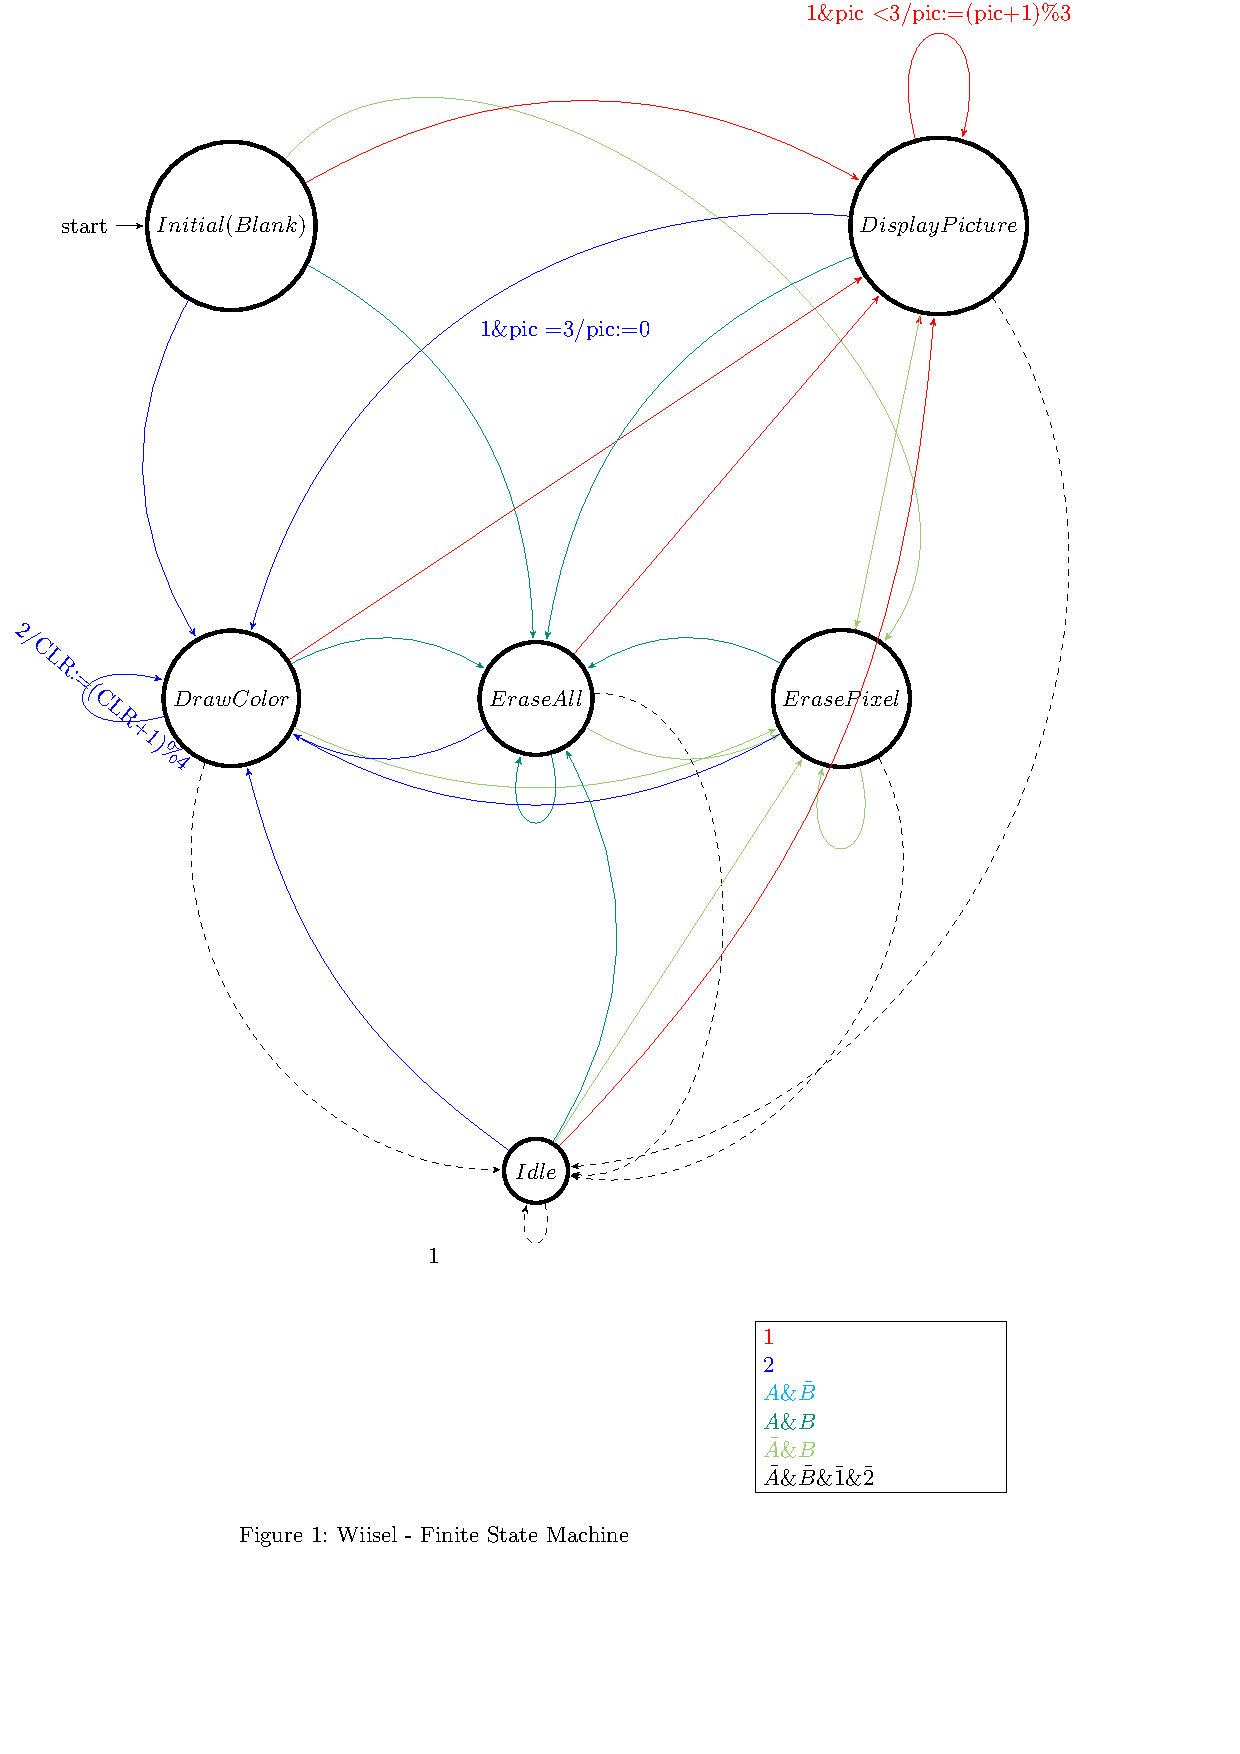
\includegraphics[width=0.9\textwidth]{fsm2.pdf}
    \caption{Model Finite State Machine}
    \label{fsm}
\end{figure*}
\end{document}
